%%%%%%%%%%%%%%%%%%%%%%%%%%%%%%%%%%%%%%%%%%%%%%%%%%%%%%%%%%%%%%%%%%%%%
%% This is a (brief) model paper using the achemso class
%% The document class accepts keyval options, which should include
%% the target journal and optionally the manuscript type. 
%%%%%%%%%%%%%%%%%%%%%%%%%%%%%%%%%%%%%%%%%%%%%%%%%%%%%%%%%%%%%%%%%%%%%
\documentclass[journal=jacsat,manuscript=article]{achemso}

%%%%%%%%%%%%%%%%%%%%%%%%%%%%%%%%%%%%%%%%%%%%%%%%%%%%%%%%%%%%%%%%%%%%%
%% Place any additional packages needed here.  Only include packages
%% which are essential, to avoid problems later. Do NOT use any
%% packages which require e-TeX (for example etoolbox): the e-TeX
%% extensions are not currently available on the ACS conversion
%% servers.
%%%%%%%%%%%%%%%%%%%%%%%%%%%%%%%%%%%%%%%%%%%%%%%%%%%%%%%%%%%%%%%%%%%%%
\usepackage[version=3]{mhchem} % Formula subscripts using \ce{}
\usepackage{comment}

%%%%%%%%%%%%%%%%%%%%%%%%%%%%%%%%%%%%%%%%%%%%%%%%%%%%%%%%%%%%%%%%%%%%%
%% If issues arise when submitting your manuscript, you may want to
%% un-comment the next line.  This provides information on the
%% version of every file you have used.
%%%%%%%%%%%%%%%%%%%%%%%%%%%%%%%%%%%%%%%%%%%%%%%%%%%%%%%%%%%%%%%%%%%%%
%%\listfiles

%%%%%%%%%%%%%%%%%%%%%%%%%%%%%%%%%%%%%%%%%%%%%%%%%%%%%%%%%%%%%%%%%%%%%
%% Place any additional macros here.  Please use \newcommand* where
%% possible, and avoid layout-changing macros (which are not used
%% when typesetting).
%%%%%%%%%%%%%%%%%%%%%%%%%%%%%%%%%%%%%%%%%%%%%%%%%%%%%%%%%%%%%%%%%%%%%
\newcommand*\mycommand[1]{\texttt{\emph{#1}}}

%%%%%%%%%%%%%%%%%%%%%%%%%%%%%%%%%%%%%%%%%%%%%%%%%%%%%%%%%%%%%%%%%%%%%
%% Meta-data block
%% ---------------
%% Each author should be given as a separate \author command.
%%
%% Corresponding authors should have an e-mail given after the author
%% name as an \email command. Phone and fax numbers can be given
%% using \phone and \fax, respectively; this information is optional.
%%
%% The affiliation of authors is given after the authors; each
%% \affiliation command applies to all preceding authors not already
%% assigned an affiliation.
%%
%% The affiliation takes an option argument for the short name.  This
%% will typically be something like "University of Somewhere".
%%
%% The \altaffiliation macro should be used for new address, etc.
%% On the other hand, \alsoaffiliation is used on a per author basis
%% when authors are associated with multiple institutions.
%%%%%%%%%%%%%%%%%%%%%%%%%%%%%%%%%%%%%%%%%%%%%%%%%%%%%%%%%%%%%%%%%%%%%

\author{Nicholas A. Tiwari}
\affiliation[Carnegie Mellon University]
{Carnegie Mellon University, Pittsburgh, PA}
\author{Andrew M. Park}
\author{Scott Blackburn}
\affiliation[Chemours]
{The Chemours Company, Newark, DE}
\author{Ashley J. Bird}
\author{Ahmet Kusoglu}
\affiliation[Lawrence Berkeley National Lab]
{Lawrence Berkeley National Lab, Berkeley, CA}
\author{Zachary W. Ulissi}
\author{Shawn Litster}
\author{Gerald J. Wang}
\email{gjwang@cmu.edu}
\affiliation[Carnegie Mellon University]
{Carnegie Mellon University, Pittsburgh, PA}

\usepackage{booktabs}

%%%%%%%%%%%%%%%%%%%%%%%%%%%%%%%%%%%%%%%%%%%%%%%%%%%%%%%%%%%%%%%%%%%%%
%% The document title should be given as usual. Some journals require
%% a running title from the author: this should be supplied as an
%% optional argument to \title.
%%%%%%%%%%%%%%%%%%%%%%%%%%%%%%%%%%%%%%%%%%%%%%%%%%%%%%%%%%%%%%%%%%%%%
\title[An \textsf{achemso} demo]
  {Effects of Ionomer Backbone Composition on Morphology and O$_2$ Transport}

%%%%%%%%%%%%%%%%%%%%%%%%%%%%%%%%%%%%%%%%%%%%%%%%%%%%%%%%%%%%%%%%%%%%%
%% Some journals require a list of abbreviations or keywords to be
%% supplied. These should be set up here, and will be printed after
%% the title and author information, if needed.
%%%%%%%%%%%%%%%%%%%%%%%%%%%%%%%%%%%%%%%%%%%%%%%%%%%%%%%%%%%%%%%%%%%%%
\abbreviations{HOPI,PFSA}
\keywords{American Chemical Society, \LaTeX}

%%%%%%%%%%%%%%%%%%%%%%%%%%%%%%%%%%%%%%%%%%%%%%%%%%%%%%%%%%%%%%%%%%%%%
%% The manuscript does not need to include \maketitle, which is
%% executed automatically.
%%%%%%%%%%%%%%%%%%%%%%%%%%%%%%%%%%%%%%%%%%%%%%%%%%%%%%%%%%%%%%%%%%%%%
\begin{document}

%%%%%%%%%%%%%%%%%%%%%%%%%%%%%%%%%%%%%%%%%%%%%%%%%%%%%%%%%%%%%%%%%%%%%
%% The "tocentry" environment can be used to create an entry for the
%% graphical table of contents. It is given here as some journals
%% require that it is printed as part of the abstract page. It will
%% be automatically moved as appropriate.
%%%%%%%%%%%%%%%%%%%%%%%%%%%%%%%%%%%%%%%%%%%%%%%%%%%%%%%%%%%%%%%%%%%%%
\begin{tocentry}

\centering
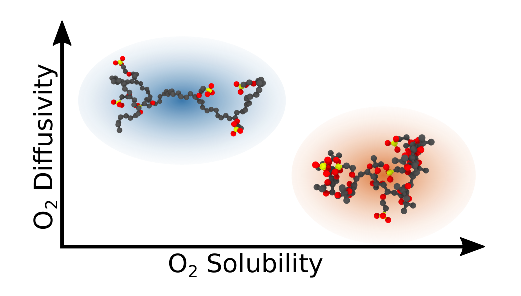
\includegraphics{tocfigure.eps}


\end{tocentry}

%%%%%%%%%%%%%%%%%%%%%%%%%%%%%%%%%%%%%%%%%%%%%%%%%%%%%%%%%%%%%%%%%%%%%
%% The abstract environment will automatically gobble the contents
%% if an abstract is not used by the target journal.
%%%%%%%%%%%%%%%%%%%%%%%%%%%%%%%%%%%%%%%%%%%%%%%%%%%%%%%%%%%%%%%%%%%%%
\begin{abstract}
Proton exchange membrane  (PEM) fuel cells are compact and lightweight fuel cells that use an acidic polymer membrane as an electrolyte. They have a lower carbon footprint than combustion engines and are not subject to the restrictively low gravimetric energy densities of modern batteries, making them ideal power sources for heavy-duty transport applications such as trucks and buses. However, resistance to oxygen transport in the ion-conductive polymer, or ionomer, that coats catalyst particles in the cell cathode has been associated with decreased cell power output and durability. In this research, we employ molecular simulation techniques to compare the oxygen transport properties between an ionomer with a PTFE backbone, similar to commercial offerings, and a recently developed high oxygen permeability ionomer (HOPI) whose backbone is comprised of dioxolane rings. We find that oxygen permeability is up to four times higher in the HOPI, owing to substantially higher oxygen solubility. 
\end{abstract}

%%%%%%%%%%%%%%%%%%%%%%%%%%%%%%%%%%%%%%%%%%%%%%%%%%%%%%%%%%%%%%%%%%%%%
%% Start the main part of the manuscript here.
%%%%%%%%%%%%%%%%%%%%%%%%%%%%%%%%%%%%%%%%%%%%%%%%%%%%%%%%%%%%%%%%%%%%%
\section{Introduction}
Proton exchange membrane fuel cells (PEMFCs) are a promising power source for heavy-duty transportation because of their relatively low operating temperatures and high power density; however, several barriers prevent their widespread adoption\cite{Cullen2021, pemfc-costing}, including degradation of the platinum catalyst, which reduces the operating efficiency and increases the lifetime operating cost of a PEMFC \cite{weber_critical_2014,braaten_studying_2020,bi_modeling_2008,ferreira_instability_2005,braaten_contaminant_2019}. Numerous strategies have been investigated to mitigate these weaknesses, including improving catalyst activity \cite{molmen_recent_2021,chandran_high-performance_2018,koh_effects_2008,he_single_2020} and developing better carbon supports \cite{ramaswamy_carbon_2020,yu_carbon-support_2009}. There has also been a considerable effort dedicated to modifying the ion-conductive polymer (ionomer), with the goal of improving gas permeability \cite{jomori_analysis_2012,Greszler_Caulk_Sinha_2012,sakai_analysis_2009,mohamed_effects_2009}. 

It is this last approach that motivates the present work, in which we investigate the relationship between ionomer morphology and oxygen permeability using molecular simulation. Ionomers used in PEMFCs are often perfluorosulfonic acid (PFSA) polymers composed of polytetrafluoroethylene (PTFE) backbones and sulfonate functionalized pendant side chains; commercially available examples of such ionomers include Nafion™, Flemion™, and Aciplex™. Such ionomers have been shown experimentally to form dense, crystalline domains in which the backbone segments are neatly stacked\cite{modestino_controlling_2012, ludvigsson_crystallinity_2000}, reducing the fractional free volume (FFV) of the ionomer, which in turn reduces gas permeability through the system. It has also been show that reducing the equivalent weight (polymer mass per ionic group) tends to lead to higher FFVs \cite{wang_evaluation_2012}, although there is evidence that proton transport is hindered at equivalent weights below 700 g/mol\cite{giffin_interplay_2013}. 

Longer side chains can also increase the free volume by reducing crystallinity; they are able to access more space in the polymer matrix, where they act as impurities, inhibiting the formation and growth of microcrystallites \cite{ghielmi_proton_2005}. However, the sulfonic groups that terminate side chains have a high affinity for the platinum catalyst, and the increased flexibility of longer side chains facilitates the adsorption of sulfonate moieties to the platinum \cite{kodama_effect_2018}. This results in a high density monolayer of sulfonates at the ionomer-platinum interface, which is difficult for O$_2$ to permeate. 

Incorporation of bulky structures into the backbone can reduce resistance to O$_2$ transport, while having only a marginal adverse effect on proton transport \cite{katzenberg_highly_2020,jinnouchi_role_2021,pinnau_gas_1996,rolfi_new_2018}. In this work, we employed molecular dynamics (MD) simulations to evaluate the differences in O$_2$ diffusivity, solubility and permeability between a high oxygen permeability ionomer (HOPI), whose backbone contains bulky dioxolane rings, and a sample PFSA chemistry that is representative of commercially available ionomers. Structural representations of these chemistries are given in Figure \ref{fig:chemcomp}. We calculated solubility and diffusivity coefficients using models of both a bulk ionomer and of an ionomer adsorbed to a platinum slab, and then investigated the effects that differences in ionomer morphology at different water contents could have on these properties. 

\begin{figure}[h!]
  \includegraphics[width=.9\linewidth]{chemcomp.png}
  \label{fig:chemcomp}
  \centering
  \caption{Molecular structures for the PFSA and HOPI studied herein. $x$ is the number of backbone units per polymer repeat unit, and $z$ is the number of polymer repeat units. Red indicates oxygen, yellow indicates sulfur, and gray indicates carbon. Fluorine occludes important geometric features, and so is not shown in these visualizations.}
  \end{figure}

The permeability of a gas $x$, $P_x$, in any polymeric membrane is described by a solution-diffusion mechanism. Permeability is the product of a diffusive (kinetic) term $D_x$ and a solubility (thermodynamic) term $S_x$:

\begin{equation}
    \label{eqn:permeability}
    P_x = S_xD_x
\end{equation}

\section{Methods}
\subsection{Water Content Measurements}
Gas permeability in a membrane varies with ambient relative humidity (RH) \cite{broka_oxygen_1997,novitski_determination_2015,schalenbach_gas_2015}. We conducted experiments to establish ionomer water content as a function of relative humidity and used these data to set the number of water molecules present in our simulations. Data are given in Figure \ref{fig:water-number}; water content is in units of moles of water per mole of sulfonate anion. A description of experimental techniques is given in the Supplementary Information. 

\begin{figure}
    \centering
    \includegraphics[width=0.9\linewidth]{humidity.png}
    \caption{Water content $\lambda$ as a function of relative humidity for PFSA (blue) and the HOPI (orange). Water content increases with RH for both the HOPI and PFSA. Water uptake is substantially higher for the PFSA between 85\% and 100\% humidity.} 
    \label{fig:water-number}
\end{figure}


\subsection{Simulations}
Equivalent weights were set to 993 g/mol and 852 g/mol for PFSA and HOPI, respectively. This corresponds to 7 backbone units and 2.33 backbone units per polymer repeat unit. While the EWs in simulations are slightly different from the EWs studied in the water uptake experiments, we expect that the difference is small enough that there will be no meaningful difference in the overall trends of the studied observables. All sulfonic groups were assumed to be ionized. Hydronium ions were added to offset the negative charge incurred by the deprotonated sulfonate groups, and were counted towards the total number of waters. Because total ionization was assumed, simulations were only be conducted at water numbers equal to or greater than 1, which corresponds to a minimum RH value of 53\%.  


Two models are developed and investigated in this research. The first is a bulk model which contains exclusively water and ionomer, and is used for diffusivity and bulk density calculations. The second is a thin-film model that contains water, ionomer, and platinum, and is used for solubility calculations. Initial configurations were generated using the Enhanced Monte Carlo (EMC) software package\cite{in_t_veld_temperature-dependent_2003}, and simulations were conducted using LAMMPS \cite{thompson_lammps_2022}.
\begin{figure}[h]
  \includegraphics[width=.9\linewidth]{systemvis.png}
  \centering
  \caption{Visualizations of the bulk and thin-film systems. Green is fluorine, red is oxygen, dark gray is carbon, yellow is sulfur and light gray is platinum. Thin-film supercells had fixed displacements of 33.2 {\AA} in the $x$ direction and 22.8 {\AA} in the $y$ direction. $z$ displacements ranged from 50 {\AA} to 58 {\AA}. Bulk supercells were cubes, with edge lengths ranging from 44 {\AA} to 47 {\AA}.}
   \label{fig:visualizations}
\end{figure}
Visualizations of both systems are given in Figure \ref{fig:visualizations}. Polymer-polymer interactions are described using the DREIDING force field \cite{mayo_dreiding_1990}, and polymer-platinum interactions are described using the force field proposed by Brunello et al. \cite{brunello_interactions_2016}. The simulations were run for 10 nanoseconds using a time step of 0.5 femtoseconds. The first nanosecond was a high temperature stage conducted at 1000 K to allow polymers to overcome kinetic barriers, the second nanosecond was an annealing stage where the temperature was reduced from 1000 K to 353 K, and the remaining time was an equilibration and data collection stage, which was conducted at 353 K. The next two sections provide detailed information on the methods used to develop bulk and thin-film models. 

\subsubsection{Bulk System}
Eight simulations, each starting from a different initial configuration, were performed at each humidity. The supercell for each simulation contained 20 polymer chains, 40 O$_2$ molecules, and a varying number of waters depending on humidity. The boundary conditions were periodic in all three dimensions. The supercells were initialized to a density of 1.6 g/cm$^3$, and the initial cell edge length ranged from 47 A to 50 A. The system was held in the NVT ensemble for the annealing and temperature reduction stages, and switched to the NPT ensemble with a pressure of 1 atm for the data collection stage. The mean squared displacement (MSD) data for O$_2$ was extracted from the final four nanoseconds of each simulation using the \texttt{compute msd/chunk} command in LAMMPS, and used to calculate the O$_2$ self-diffusion coefficient at different water numbers. The self-diffusion coefficients were calculated via the Einstein relation, given in Equation \ref{eqn:einstein}. 

\begin{equation}
  \label{eqn:einstein}
  D_{O_2} = \frac{1}{6} \lim_{t \to \infty} \frac{d}{dt} \frac{1}{N} \sum_{i=1}^{N} \langle|r_{O_2}(t) - r_{O_2}(0)|\rangle^2 
\end{equation}

$D_{O_2}$, the oxygen self-diffusion coefficient, was calculated by fitting a linear model to average mean squared displacement data, which is given by $\frac{1}{N} \sum_{i=1}^{N} \langle|r_{O_2}(t) - r_{O_2}(0)|\rangle^2 $ in Equation \ref{eqn:einstein}. The model was fitted using linear least-squares regression. Density of the bulk was calculated by averaging the density of the supercell for the final four nanoseconds of the data collection stage. 
\subsubsection{Thin-film System}
A single NVT simulation was conducted at each humidity. Each supercell contained eight polymer chains, and a varying number of waters depending on the humidity. The liquid phase in each supercell was initialized to the bulk density at that humidity, and the system was assumed periodic only in the $x$ and $y$ directions. In the $z$ direction, the system was constrained by the platinum slab at the bottom of the box and a harmonic wall boundary condition at the top of the box, implemented using the \texttt{wall/harmonic} fix in LAMMPS. The functional form of the harmonic boundary condition is given in Equation \ref{eqn:harmonic}. 
\begin{equation}
    \label{eqn:harmonic}
    U = k(r-r_c)^2 \qquad r < r_c
\end{equation}

Where $U$ is the potential energy, $r$ is the distance from a particle to the boundary condition, $k$ is the spring constant, which was set to 600.0 kcal/mol, and $r_c$ is the cutoff distance, which was set to 4 angstroms below the top of the supercell. The platinum slab was immobilized to ensure that platinum atoms did not migrate out of the supercell during the simulation. The solubility of oxygen in the liquid phase was determined using the final nanosecond of each simulation, where it was assumed that the supercell was in chemical equilibrium with gas phase O$_2$. To calculate the solubility, we assumed that the supercell was in chemical equilibrium with an oxygen gas phase. This was achieved via the GCMC package in LAMMPS, which performs grand canonical Monte Carlo insertions with a fictitious ideal gas reservoir, as described by Frenkel and Smit \cite{frenkel_understanding_2002}. Solubility was determined by counting the number of O$_2$ molecules present in the supercell at the time steps where GCMC exchanges were attempted, and averaging this count over the whole GCMC run.

\section{Results and discussion}
\subsection{Oxygen Self-Diffusion Coefficient}
Self-diffusion coefficients are given as a function of water number in Figure \ref{fig:diffusivity}. At less than 75\% humidity, the HOPI exhibits higher diffusivity. Above this threshold, the diffusivity of O$_2$ in PFSA quickly outpaces the HOPI. A possible explanation lies in morphological differences between the two chemistries at high water numbers. Experiments by Inaba et. al. indicate that O$_2$ preferentially orients at interfaces between hydrophilic and hydrophobic regions \cite{inaba_oxygen_1993}, meaning that continuity of hydrophilic domains has a strong effect on O$_2$ diffusivity. 
\begin{figure}[h!]
  \includegraphics[width=0.9\linewidth]{diffusivity.png}
  \centering
  \caption{Oxygen self-diffusion coefficients as a function of water number for the HOPI (orange) and PFSA (blue). Error bars are represent a 95\% confidence interval.}
\label{fig:diffusivity}
\end{figure}

To gain insight into the morphological characteristics of both polymer chemistries, we use the cluster analysis tool provided in OVITO \cite{stukowski_visualization_2009}. Here, a particle is part of a cluster if it is within 3 {\AA} of any other particle that is part of that same cluster. Figure \ref{fig:clustering} gives snapshots of hydrophilic clusters in bulk phase HOPI and PFSA simulations at 85\% humidity. PFSA contains fewer, larger clusters compared to the HOPI; there are 18 hydrophilic clusters in PFSA and 34 hydrophilic clusters in HOPI. We expect that the long, channel-like clusters in the PFSA act as corridors along which O$_2$ can move, while the short, fragmented clusters of the HOPI restrict movement. The result is a disparity in the self-diffusion coefficient between the HOPI and PFSA, particularly at high humidities. 
\begin{figure}[h!]
  \includegraphics[width=.9\linewidth]{clustering.png}
  \centering
  \caption{Water clustering in PFSA and HOPI. Water molecules of the same color are part of the same cluster.}
  \label{fig:clustering}
\end{figure}

\subsection{Oxygen Solubility}
O$_2$ solubility in the ionomer and the density determined from the bulk calculations are given as a function of the water content in Figure \ref{fig:solubility}. The negative correlation between O$_2$ solubility and water content is probably attributable to density and morphological differences. The lower bulk densities exhibited by the HOPI indicate a higher fractional free volume, some of which is accessible to O$_2$. As the number of water increases, O$_2$ is displaced by the water that fills void spaces. At the interface, this effect is magnified by strong interactions between O$_2$ and platinum. Figure \ref{fig:violin-plots} gives the probability distributions for the location of an O$_2$ molecule at a given distance from the platinum surface. The vertically split violins are composed of two kernel density estimations: one for PFSA, and the other for HOPI.  Probability distribution functions at the same humidity share a common scaling. 

\begin{figure}[h!]
  \includegraphics[width=\linewidth]{densitysolubility.png}
  \centering
  \caption{(Left) oxygen solubility for PFSA and HOPI as a function of water number, and (right) bulk density of hydrated PFSA and HOPI as a function of water number.}
    \label{fig:solubility}
\end{figure}

\begin{figure}[h!]
  \includegraphics[width=.9\linewidth]{violinplotedited.png}
  \centering
  \caption{Violin plots for O$_2$ distribution in PFSA and HOPI at different humidities. Probability density functions are set to zero at positions where there is no oxygen present.}
    \label{fig:violin-plots}
\end{figure}

At most humidities, there is a notable peak towards the base of the probability distribution. The high concentration of oxygen at this location is probably due to strong enthalpic interactions between oxygen and platinum. As humidity increases, this peak increases slightly. At high humidity, water forms a monolayer in regions at the interface that are not occupied by the polymer. O$_2$ cannot adsorb directly to the catalyst, and is relegated to a less dense region of the liquid phase that is above the water monolayer. Figure \ref{fig:o2-slab} presents visualizations of HOPI models at two humidities. There are far fewer water adsorbed on the catalyst surface at low humidities, leaving more space for O$_2$. No O$_2$ is adsorbed at 85\% humidity; any O$_2$ present in the system is at least the thickness of the water monolayer on the surface. 
\begin{figure}[h!]
  \includegraphics[width=.9\linewidth]{adsorbatevis.png}
  \centering
  \caption{Visualizations of trajectories of the HOPI model at two humidities. The color convention is the same as in Figure \ref{fig:visualizations}, except for O$_2$, which is indicated with light blue. All particles shown are within seven angstroms of the platinum slab.} 
  \label{fig:o2-slab}
\end{figure}

\subsection{Oxygen Permeability}
Oxygen permeability in PFSA and HOPI is shown in Figure \ref{fig:permeability}. The permeability was calculated using the solubility and diffusivity data presented in the preceding sections, and Equation \ref{eqn:permeability}. The substantial difference in permeability at low water contents is primarily due to high O$_2$ solubility in the HOPI. We expect that this is a result of the higher free volume fraction mentioned, which we believe to be present in the HOPI.  
\begin{figure}[h!]
  \includegraphics[width=.9\linewidth]{perm_d2020.png}
  \centering
  \caption{Permeability of oxygen in the HOPI and sample PFSA. At the lowest water content, permeability in the HOPI is approximately four times high than the sample PFSA.} 
  \label{fig:permeability}
\end{figure}

\section{Conclusions}
Simulations of a sample PFSA chemistry similar to commercially available ionomers, and a modified high oxygen permeability ionomer (HOPI) were conducted to gauge the effects of backbone chemistry on O$_2$ solubility, diffusivity and permeability. The O$_2$ self-diffusion coefficient is larger for HOPI at low water numbers, but is quickly outpaced by PFSA as water number increases. The disparity is likely attributable to morphological differences, specifically differences in hydrophilic clustering between ionomer chemistries. Clustering analysis at high humidities indicates the presence of long, continuous hydrophilic channels in PFSA along which O$_2$ can diffuse. In contrast, small fragmented clusters in the HOPI restrict the movement of O$_2$. O$_2$ solubility in HOPI is higher than that of PFSA at all water numbers. We expect this to be an outcome of the lower bulk density in the HOPI. At low water numbers, most of the O$_2$ is concentrated close to the catalyst, due to strong enthalpic interactions between O$_2$ and platinum. At high water numbers, more water is available to fill void spaces, displacing O$_2$ and lowering the overall solubility. This effect is magnified at the interface, as a result of the strong interactions between water and platinum. Adsorbed water molecules form a monolayer that precludes adsorption of O$_2$ molecules. 

Probably the most important qualitative result of this work is that the incorporation of bulky dioxole groups into the ionomer backbone results in higher O$_2$ solubility. This increase in solubility has a disproportionate and desirable effect on the permeability of O$_2$ in the thin film. We expect that future work on the HOPI will focus on making chemical modifications that improve solubility, and diffusivity. Future work will involve a more systematic investigation of specific chemical segments of ionomer. While equivalent weight, side chain length, and side chain composition are expected to have an impact on the thin film's morphology and ability to transport O$_2$, how these design variables will interplay to affect O$_2$ transport is largely unknown. 

\begin{suppinfo}
Experimental methods used to collect water uptake data in Figure \ref{fig:water-number} are described in the Supporting Information.
\end{suppinfo}

\bibliography{OxygenPermeabilityPaper}

\end{document}